本文提出了一种从软件开发问答网站Stack Overflow中抽取出API描述性知识的方法。本章首先会详细介绍本文定义的API描述性知识概念模型,并给出一个运行示例用于展示本文方法流程。然后,本章会对API描述性知识抽取方法中的每个步骤进行详细说明。本抽取方法的流程概览如图\ref{图3-1}所示:

\begin{figure}[htb]
    \centering
    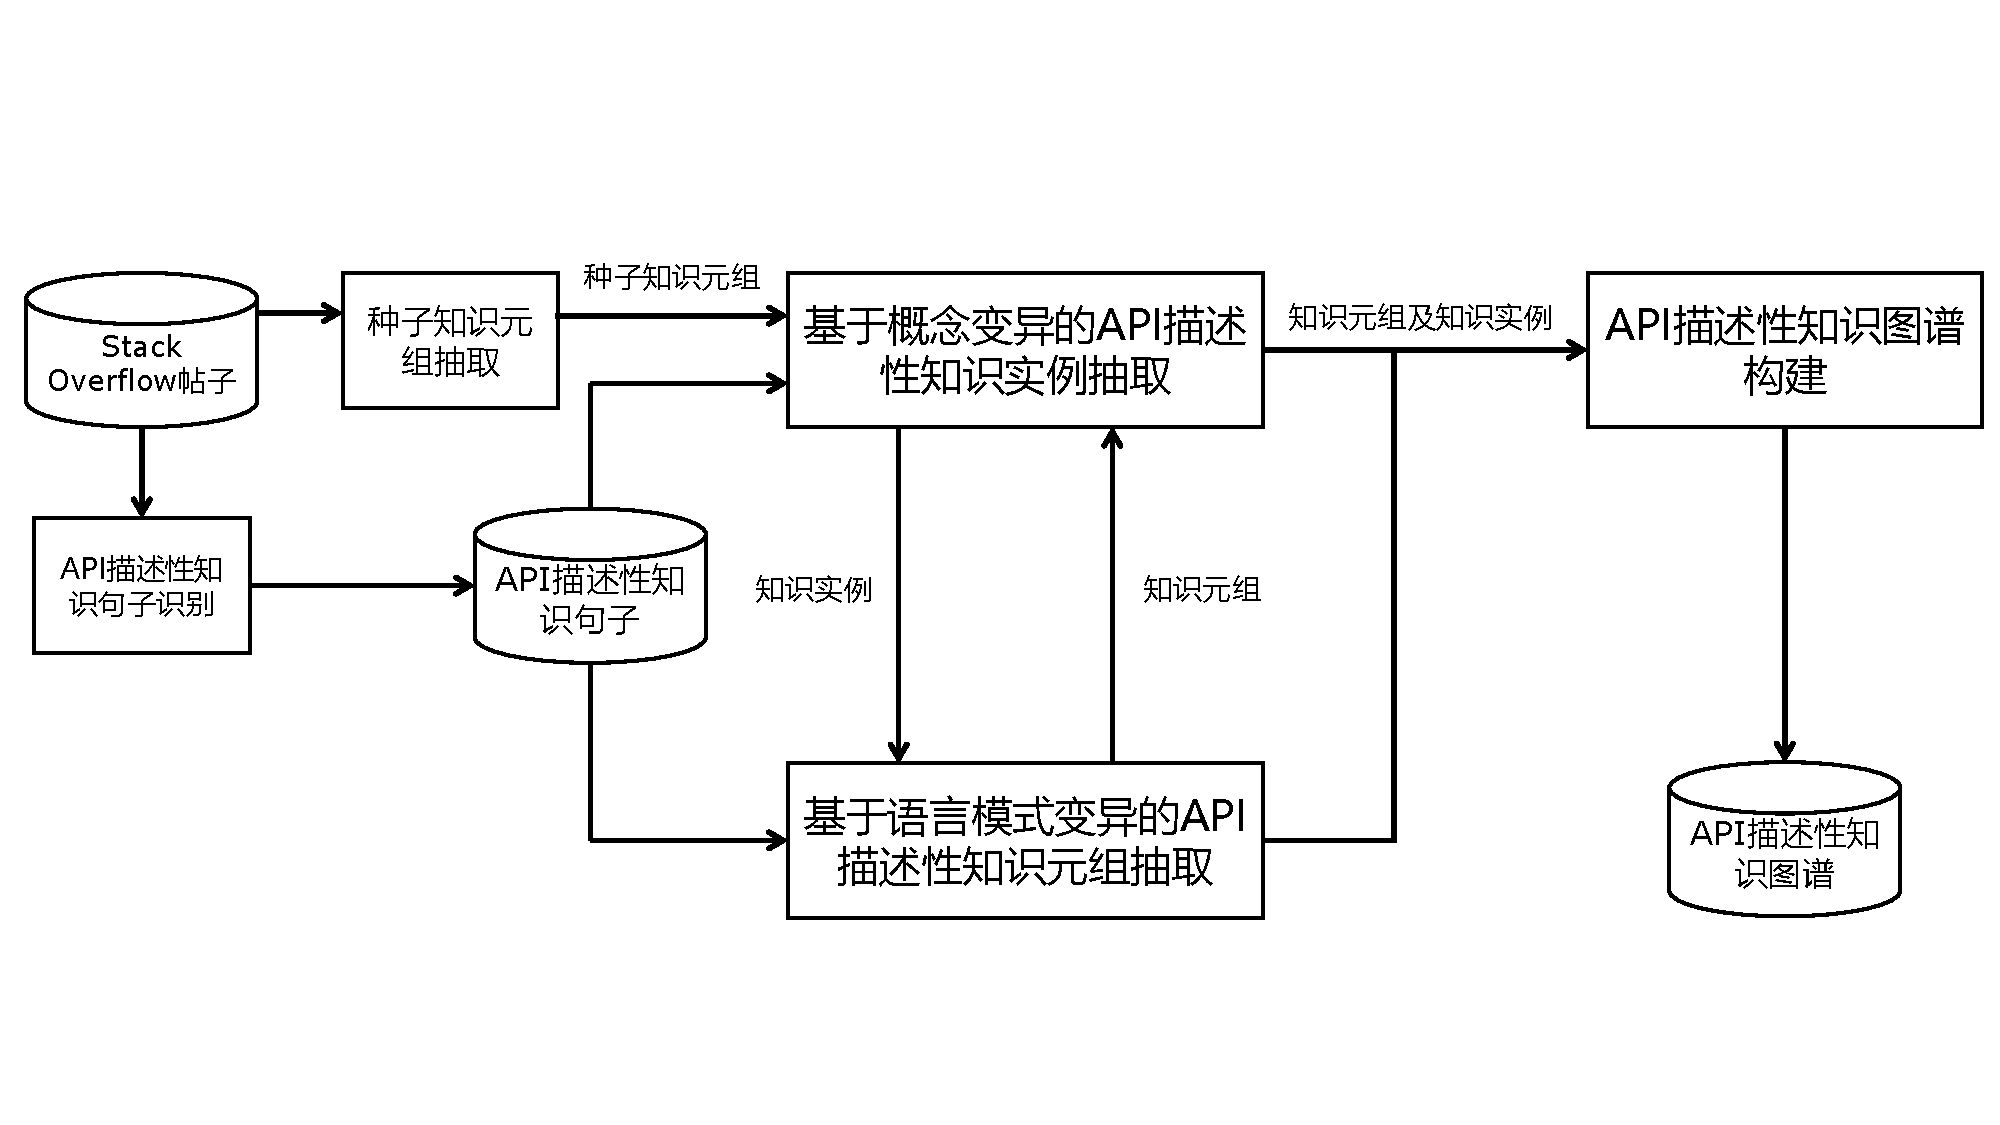
\includegraphics[width=\textwidth]{image/overview.pdf}
    \caption{API描述性知识抽取流程概览} 
    \label{图3-1} 
\end{figure}

本文提出的方法可以分为五个步骤:
\begin{enumerate}
    \item API描述性知识句子识别。该步骤从Stack Overflow网站的数据中抽取过滤出用于抽取API描述性知识的语料库,详细内容在章节3.3中说明。该步骤的流程如下:
    \begin{enumerate}
        \item Stack Overflow帖子获取。从完整的Stack Overflow网站数据库中设置一定的条件进行筛选,得到用于生成语料库的帖子集合。
        \item API描述性知识句子候选抽取。使用优化过的spaCy工具对上一步中得到的帖子的文本进行分句,并进行一系列基于正则规则的过滤,得到包含有API提及的句子作为候选。
        \item API描述性知识句子分类。使用一个训练好的fastText文本分类器,对上一步中得到的带有API提及的句子进行分类,将分类出来的API描述性知识句子作为用于抽取API描述性知识的语料库。
    \end{enumerate}
    \item 种子知识元组抽取。该步骤根据本方法指定的规则,从API描述性知识句子中抽取出知识元组,作为下一步骤的输入。详细生成规则在章节3.4中介绍。
    \item 基于概念变异的API描述性知识实例抽取。该步骤根据给定的API描述性知识元组进行知识抽取,详细的介绍在章节3.5中。本步骤的流程如下:
    \begin{enumerate}
        \item 知识元组过滤。对于给定的API描述性知识元组,本方法设定了一系列规则对其进行过滤,筛选掉其中质量不高的知识元组。
        \item 知识元组变异。对上一步中过滤后的知识元组,将它们根据定义好的一系列变异方式进行修改变异,得到更多的知识元组,这些变异得到的知识元组是潜在的API描述性知识。
        \item 知识元组匹配。使用种子API描述性知识元组和变异得到的API描述性知识元组在语料库中进行匹配,获得API描述性知识实例句子。    
    \end{enumerate}
    \item 基于语言模式变异的API描述性知识元组抽取。该步骤根据给定的API描述性知识实例句子进行知识抽取,得到更多API描述性知识元组。详细流程见章节3.6。其子步骤如下:
    \begin{enumerate}
        \item 语言模式抽取。从上一步中匹配得到的API描述性知识实例句子中总结出这个句子的语言模式,这个语言模式可能代表了人们常用于描述这种类型的知识的习惯用语。
        \item 语言模式变异。得到语言模式后,通过设定好的规则对其进行泛化修改,得到若干变异后的语言模式。
        \item 语言模式匹配。使用上一步中得到的变异语言模式在语料库中进行匹配,找到那些符合语言模式的句子,这些句子也是API描述性知识实例句子。从这些句子中可以总结出新的API描述性知识元组。
    \end{enumerate}
    步骤3和步骤4的执行逻辑如算法1所示。步骤3输出的API描述性知识实例就是步骤4的输入数据,而步骤4输出的API描述性知识元组则可以作为步骤3的输入数据。通过迭代地执行步骤3和步骤4,本方法可以从语料库中不断地抽取出API描述性知识。迭代抽取的程序逻辑如算法2所示。
    \item API描述性知识图谱构建。将上述步骤中抽取得到的API描述性知识以及API描述性知识实例句子以图谱节点的形式保存到知识图谱中,并为它们构建节点之间的关系。详细的知识图谱设计见章节3.7。
\end{enumerate}

\floatname{algorithm}{算法}  
\renewcommand{\algorithmicrequire}{\textbf{输入:}}  
\renewcommand{\algorithmicensure}{\textbf{输出:}}  
\begin{algorithm}  
    \caption{API描述性知识抽取的单步流程} 
    \begin{algorithmic}[1] %每行显示行号  
        \Require $currentSeedList$种子API描述性知识元组,$sentenceList$语料库,$result$上一轮迭代抽取得到的结果
        \Ensure $result$新一轮知识抽取得到的结果
        \Function{runForOneStep}{$currentSeedList, sentenceList, result$}  
            \State 过滤currentSeedList和sentenceList
            \State currentSeedList \gets currentSeedList变异得到的知识元组
            \State InstanceList \gets currentSeedList和sentenceList匹配得到的知识实例
            \State patternList \gets 从InstanceList中抽取并变异得到的语言模式
            \State patternInstancePair \gets PatternList和sentenceList匹配得到的知识实例
            \State newSeedList \gets 从patternInstancePair中抽取出的知识元组
            \State 将上述结果保存到result中
            \State \Return{$result$}
        \EndFunction  
    \end{algorithmic}  
\end{algorithm} 

\floatname{algorithm}{算法}  
\renewcommand{\algorithmicrequire}{\textbf{输入:}}  
\renewcommand{\algorithmicensure}{\textbf{输出:}}  
\begin{algorithm}  
    \caption{API描述性知识抽取的总体流程}  
    \begin{algorithmic}[1] %每行显示行号  
        \Require $seedList$种子API描述性知识元组,$sentenceList$语料库,$maxStep$最大迭代次数,$saveByStep$每多少步保存一次  
        \Ensure $result$保存了API描述性知识抽取结果的Snowball对象  
        \Function {run}{$seedList, sentenceList, maxStep, saveByStep$}  
            \State result \gets []
            \For{i = 1 \to maxStep+1}
                \If {i == 1}
                    \State currentSeedList \gets seedList
                \Else
                    \State currentSeedList \gets 上一轮抽取得到的API描述性知识元组
                \EndIf
                \State result \gets \Call{runForOneStep}{$currentSeedList, sentenceList, result$}
                \If {i \% saveByStep == 0}
                    \State 将result保存到本地
                \EndIf
            \EndFor
            \State 将result保存到本地
            \State \Return{$result$}  
        \EndFunction  
    \end{algorithmic}  
\end{algorithm} 

\section{API描述性知识概念模型}
通过观察Stack Overflow中与API相关的讨论帖子,以及对帖子中带有API知识的句子进行分析,本文定义了一个概念模型,用于描述本文所定义的API描述性知识及其相关概念
。
图\ref{图3-2}为本文定义的API描述性知识概念模型。本文抽取得到的API描述性知识来自于Stack Overflow中与API相关的讨论。其中,API相关讨论包含了API相关的问题以及这些问题的回答,而与API相关的问题回答为本文提供了API描述性知识句子。API描述性知识句子是一个包含了与API功能、API特性或API表现相关的知识的句子。本方法能够从一个API描述性句子中抽象出一个API描述性知识元组,这个知识元组由若干个API知识元素组成。API知识元素分为4种类别,分别是API元素,动作,目标对象以及特性。除了API元素以外,其他三种API知识元素的分类依据是词语的词性,本文将动词词性的知识元素视为动作类型,将名词词性的知识元素分为目标对象类型,将形容词与副词词性的知识元素分为特性类型。

\begin{figure}[htb]
    \centering
    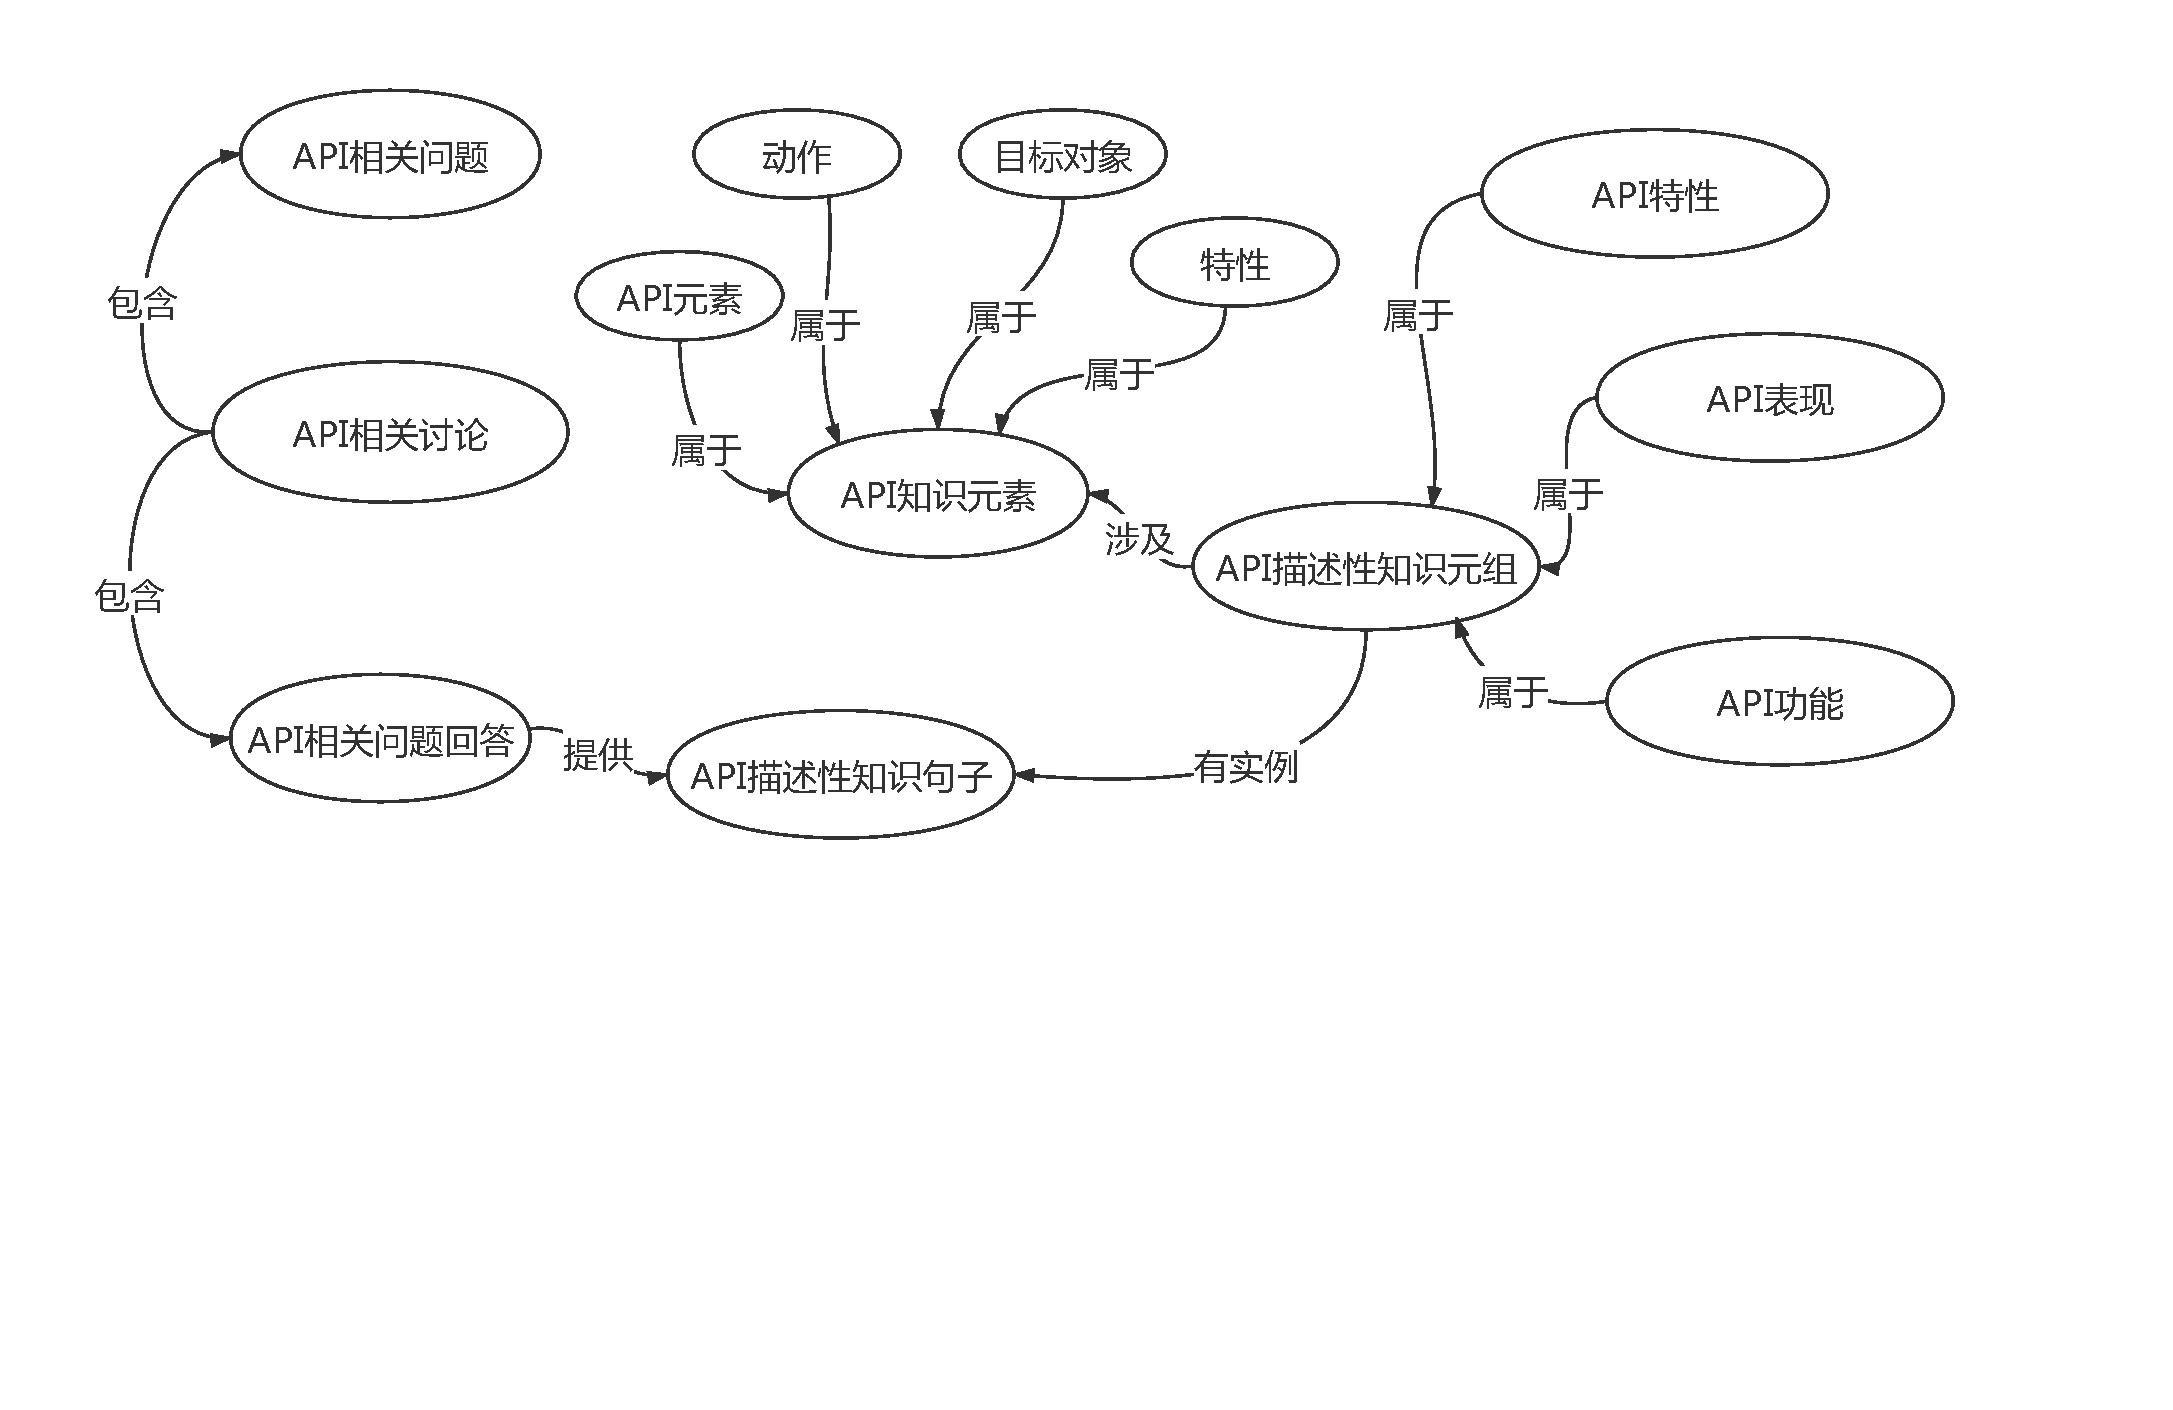
\includegraphics[width=\textwidth]{image/structure.pdf}
    \caption{API描述性知识相关概念模型} 
    \label{图3-2} 
\end{figure}

举例来说,一个API描述性知识句子:“The StringBuffer class is thread-safe.”,从这个句子中可以抽象出一个API描述性知识元组:<API:[StringBuffer], Characteristic:[thread-safe]>,它包含一个指明当前知识所属API的API元素,以及一个特性类型的API知识元素Characteristic。

根据一个API描述性知识元组所包含的API知识元素类型不同,API描述性知识也被分为三种类型,分别是API特性、API表现以及API功能。当一个知识元组仅包含特性类型的知识元素时,它会被分类为描述API特性的知识,如上一段话中所举的例子,就是一个API特性知识;当一个知识元组包含了动作和目标对象类型的知识元素时,它将被视为一个API功能类型的API描述性知识。举例而言,从句子“removeFirst() : Remove the first element in the list.”中,可以抽象出一个知识元组:<API:[removeFirst()], Action:[remove],Object:[the first element]>,这个知识元组是被分类为API功能的知识;最后,当一个知识元组包含了动作和特性知识元素时,它会被分类成描述API表现的知识,比如从句子“You can also use the javax.swing.Timer to hide this popup automatically.”中,可以抽象出一个API表现类型的知识元组<API:[javax.swing.Timer],Action:[hide],Characteristic:[automatically]>,它会被分类为API特性类型。

\section{运行示例}
本小节会使用一个API描述性知识元组作为示例,展示出本方法抽取流程的一次迭代过程,以及抽取过程中各步骤的输出。

本文首先在语料库中人工抽取出高质量的API描述性知识元组作为迭代的种子知识元组,例如,从句子“The StringBuffer class is thread-safe”中提取出知识元组<API:[StringBuffer], Characteristic:[thread-safe]>。

在每一轮迭代的开始,首先对种子进行过滤,过滤掉质量较低的种子,防止错误传递。

对剩下的高质量种子,本方法使用预设的规则对这些种子知识元组进行修改,得到一系列变异过的知识元组。例如,从知识元组<StringBuffer, thread-safe>可以变异得到一个新的知识元组<StringBuffer, synchroinzed>。这些变异得到的API描述性知识元组是潜在的可能可以从语料库中被抽取出来的API描述性知识实例的抽象表示。

变异完成后,使用这些知识元组(包括种子知识元组和变异知识元组)在语料库中进行匹配,以找到这些知识元组的实例句子。在本例子中,语料库中的句子“Each method in StringBuffer is synchronized”可以作为变异得到的知识元组<StringBuffer, synchronized>的一个实例被抽取出来。这个被抽取出来的API描述性知识实例可以用于生成这种知识的语言模式。在本示例中,上述实例包含的元素会被标注出来,进而得到“Each method in (API)[StringBuffer] is (Characteristic)[synchronized]”。

下一步是基于语言模式的变异。对上述匹配得到的API描述性知识实例,本方法抽取出其中的语言模式,并对模式中的原知识元组中的元素所在位置的词语进行变异,从而从一个已有的知识实例中生成若干可能可以代表这一知识形式的语言模式。例如,API描述性知识实例“Each method in (API)[StringBuffer] is (Characteristic)[synchronized]”可以变异得到新的句子模式“Each method in (API)[StringBuffer] is (Characteristic)[ADJ]”。其中,“[ADJ]”代表了一个词语通配符,表示可以匹配上任何一个形容词性或副词词性的词语及短语。语言模式使用新的句子模式在语料库中进行匹配,找到匹配的实例句子后,可以从中抽取出新的API描述性知识元组。例如,使用上述句子模式,可以匹配出句子“Each method in StringBuffer is ineffective”,从中可以提取出新的API描述性知识元组<API:[StringBuffer], Characteristic:[ineffective]>。

这样就完成了本方法的一轮迭代抽取流程。而在下一轮的知识抽取中,新的API描述性知识元组<API:[StringBuffer], Characteristic:[ineffective] >会作为下一轮迭代抽取的种子,继续进行变异、匹配。


\section{API描述性知识句子识别}
在执行API描述性知识的抽取流程之前,本方法需要准备好用于抽取知识的语料库,以及作为抽取流程起点的种子知识元组。本节将会介绍本文是如何从Stack Overflow中识别出API描述性知识句子的。图\ref{图3-3}展示了一个Stack Overflow与API讨论相关的问答帖子,以及在回答中包含的一个API描述性句子。

\begin{figure}[htb]
    \centering
    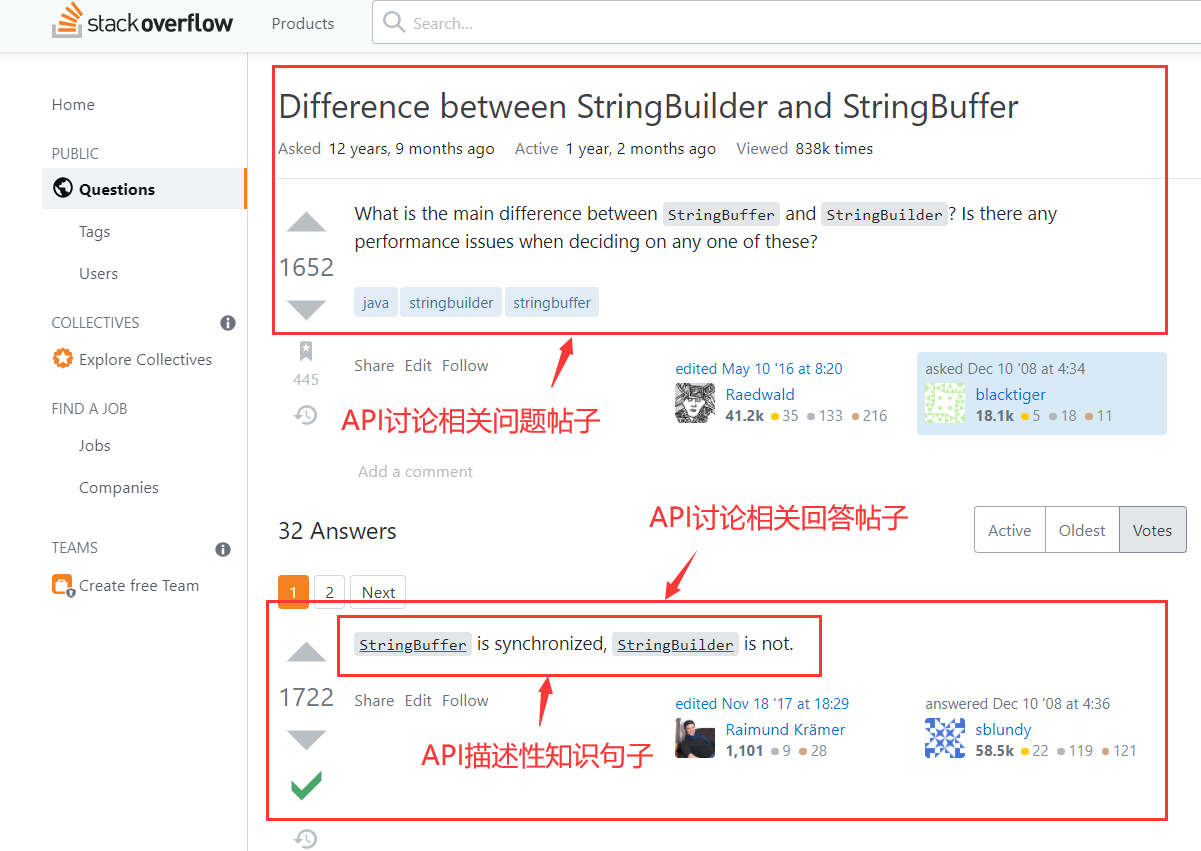
\includegraphics[width=\textwidth]{image/so.png}
    \caption{Stack Overflow中的API描述性知识句子示例} 
    \label{图3-3} 
\end{figure}

\subsection{Stack Overflow帖子获取}
本工作中进行API描述性知识抽取的语料库来自Stack Overflow。Stack Overflow官方会定期将论坛中的所有帖子数据打包,并公开发布以供学者研究(本文所使用的帖子数据是Stack Overflow官方于2021年3月发布的数据)。当然,Stack Overflow上的帖子数量过于庞大,而且并不是每一个帖子都具有被抽取的价值。因此,本方法设定了以下条件作为筛选,从Stack Overflow的所有帖子中找到符合条件的帖子作为抽取API描述性知识句子的来源:

\begin{itemize}
    \item 帖子是一个回答类型的帖子。通常,对于一个API的讨论更有可能出现在一个问题的回答中。
    \item 帖子的得分大于0。如果帖子的得分大于0,那就说明至少有一位其他用户对这篇回答持支持态度,也就意味着该回答有被抽取的价值。
    \item 帖子的标签列表中包含<java>标签。在今天,Java仍然是世界上应用最广泛的编程语言之一,开发者对Java语言相关的API知识需求很高,且Java标签是Stack Overflow上最热门的标签之一,这保证了本文语料库的规模。
\end{itemize}

\subsection{API描述性知识句子候选抽取}
对于一个含有API描述性知识的句子而言,这个句子中既有可能直接出现一个API的提及,也可能该API是在上下文中已经出现过,而在该句子中只有代词指代。显然,包含API描述性知识的句子并不一定包含API提及,但包含API提及的句子更有可能是一个包含API描述性知识的句子。因此,对于上一步中筛选得到的帖子中的所有句子,可以在其中筛选出带有API提及的句子作为候选,这些句子更有可能抽取出API描述性知识。

在筛选出帖子后,本方法对帖子进行分句。分句时,软件工程领域相关文本的一些特点可能会对分句产生影响,经过人工的观察,我们发现常见的会对文本分句造成影响的情况如下:

\begin{itemize}
    \item 一个带有包名的类名提及可能会被错误地分句。如句子“Think about \\java.lang.ThreadLocal , adding dynamic field to threads.”,可能会被分成“Think about java.lang.”和“ThreadLocal, adding dynamic field to threads.”两个句子。
    \item 一个带有参数的API提及可能会被错误地分句。如句子“currentThread() is the thread that is interrupting, not being interrupted.”可能会被错误地断成“currentThread(”和“) is the thread that is interrupting, not being interrupted.”两个句子。
    \item 某些连接符号可能会被错误的分句。如句子“HashMap is fast-fail.”可能会被分成“HashMap is fast-”和“fail.”两个句子。
\end{itemize}

本方法使用了spaCy工具对文本进行分句处理,如前文章节2.4.1所述,spaCy的可拓展性非常强,允许用户对自然语言处理中的任何一个环节进行定制化修改。为了避免分句错误对语料库带来的负面影响,本方法修改了spaCy的分句模块,使之在遇到上述情况时能够分割出符合需求的句子。

由于一个帖子中可能存在着代码片段,所以在分句之前,还需要对帖子文本中的代码片段进行一些处理。对于文本中存在的代码片段,本方法使用占位符$-CODE-$对其进行替换,避免了文本中的代码片段对当前API元素识别以及后续抽取流程的影响。

API提及包括函数名、类名以及一系列它们的变种,如带有类名的函数名提及、带有参数名的函数名提及、带有包名的类名提及等等。用户在编写
帖子时,还有可能对一个 API 名进行简写,如当提及一个带有参数的函数名时,
忽略掉参数的内容,只在函数名后加上一对圆括号。经过人工观察,本方法总结出了4个正则表达式,用于从句子文本中找到这些API提及。详细的正则表达式如表\ref{表3-1}所示。使用正则表达式匹配得到的带有API提及的句子就是API描述性知识句子的候选。

\begin{table}[h]
    \centering
    \caption{匹配API提及的正则表达式}
    \label{表3-1}
    \begin{tabular}{|l|l|}
        \hline
        \multicolumn{1}{|c|}{正则表达式}                                                                                  & \multicolumn{1}{c|}{匹配的API提及类型}                                                             \\ \hline
        ({[}a-z{]}+\textbackslash{}.)*{[}A-Z{]}{[}a-z{]}+\textbackslash{}.{[}a-z{]}+({[}A-Z{]}{[}a-z{]}+)*(\textbackslash(\textbackslash S*\textbackslash))? & \begin{tabular}[c]{@{}l@{}}一个带有完整包名、类名\\ 以及方法名的API提及,\\ 结尾的参数列表可以省略\end{tabular}            \\ \hline
        (({[}A-Za-z{]}{[}a-z{]}+)+\textbackslash{}.)?{[}a-z{]}+{[}A-Z{]}{[}a-z{]}+(\textbackslash(\textbackslash S*\textbackslash))?                         & \begin{tabular}[c]{@{}l@{}}一个带有类名和方法名的\\ 驼峰式命名提及,也可以\\ 匹配上类中的对象,结尾\\ 的参数列表可以省略\end{tabular} \\ \hline
        ({[}a-z{]}+\textbackslash{}.)+({[}A-Z{]}{[}a-z{]}+)+(\textbackslash(\textbackslash S*\textbackslash))?                                               & \begin{tabular}[c]{@{}l@{}}一个带有包名的类名提及,\\ 结尾的参数列表可以省略\end{tabular}                          \\ \hline
        ({[}A-Z{]}{[}a-z{]}+)+(\textbackslash(\textbackslash S*\textbackslash))                                                                              & \begin{tabular}[c]{@{}l@{}}一个带有参数列表的类名\\ 提及,表示这是一个构造\\ 函数\end{tabular}                      \\ \hline
    \end{tabular}
\end{table}

\subsection{API描述性知识句子分类}
为了提高本方法抽取API描述性知识的效率和准确率,本文使用了基于机器学习的文本分类技术对这些句子进行进一步的过滤。对上一步中得到的所有带API提及的句子随机抽样,并人工对它们进行标注,标注这些句子是否为一个包含API描述性知识的句子。使用这些标注数据,可以训练出一个文本分类器,用于将所有带有API提及的句子进行分类,最后只使用被分类器分类为带有API描述性知识的句子作为信息抽取的语料库,通过这种过滤方式让语料库中的句子包含API描述性知识的概率更大。

在分类之前,还需要对候选句子进行处理。由于句子中存在的API提及的词频相比其他自然语言词语低得多,这会导致分类器训练集的词表变得非常稀疏,从而严重影响分类效果。因此,本文将API描述性知识句子候选中的API提及全部使用占位符$-API-$替换,并将句子和替换下来的AP提及一起保存下来。

最后,通过文本分类技术得到的API描述性知识句子就是本方法抽取知识的语料库。

\section{种子知识元组抽取}
基于概念变异的API描述性知识实例抽取步骤需要少量的种子知识元组作为初始输入。因此,本文制定了一些规则来从一个API描述性知识句子中抽取出抽象化的API描述性知识元组。

首先,一个带有API描述性知识的句子必然包含一个API提及,这个API提及会作为API描述性知识的API元素被抽取出来。如果句子中存在一个将API提及作为宾语的动词/动词短语,或者存在一个作为API提及的谓语的动词/动词短语,那么这个动词/动词短语会作为知识元组中的动词元素被抽取出来。当API元素在句子中作为主语,且存在一个被抽取出来作为动词元素的短语时,这个句子的宾语也会作为目标对象类型的元素被抽取出来。最后,当句子中存在一个副词或形容词词性的短语用于修饰API元素时,它将会作为特性类型的元素被抽取出来。

\section{基于概念变异的API描述性知识实例抽取}
在这一步骤中,本方法将种子知识元组经过过滤、变异以及匹配三个子步骤,来从语料库中抽取出新的API描述性知识。
\subsection{知识元组过滤}
本文的知识抽取思路是基于自举思想的方法,通过迭代抽取的方式,让抽取出来的API描述性知识像滚雪球一样越滚越大,越抽越多。但是在这种抽取方式中,如果抽取出了一个错误的信息,那么就可能会匹配上错误的文本,生成错误的语言模式,继而在下一轮抽取过程中生成更多错误的结果。因此,在每一轮迭代抽取之前,本方法需要对抽取用到的种子进行过滤,去除那些可能引起雪崩式错误的种子。

过去的自举抽取信息方法,如章节2.3介绍的Snowball和NELL等系统的过滤方式是通过计算信息元组的置信度来实现的,一个元组的置信度由它包含的元素在整个语料库中出现的词频和生成它的模式的个数决定的。但在本文中,由于生成语料库的时候已经使用了一个文本分类器进行过滤,可以预见到本方法对于语料库的覆盖度是比较高的,甚至在分类器准确率极高的情况下,每一个语料库中的句子都可能可以抽取出一个API描述性知识元组来,所以计算置信度来进行过滤的方式在本方法中并不适用。在实践中也发现了如果使用置信度进行过滤,质量较差的API描述性知识元组的置信度得分与质量较好的API描述性知识元组的置信度并没有显著差异,甚至可能得分更高。

因此,本文在人工观察了一些质量较差的API描述性知识元组后,总结出了一些规则来进行过滤:

\begin{itemize}
    \item 词性过滤。API描述性知识元组中的元素只能是名词词性、动词词性和形容词词性。
    \item 词频过滤。本方法统计了语料库中所有词语出现的词频,对于那些词频极高或者词频极低的元素不予采用。
    \item 长度过滤。由于元素可能以词组的形式存在,且流程后面的模式匹配环节也支持多单词匹配一个元素,所以本方法对元素的长度进行了限制,使得一个元素的长度不能超过4个单词。
\end{itemize}

通过设定以上规则进行过滤,可以得到一些质量较高的API描述性知识元组来进行匹配。

除了过滤知识元组以外,本步骤还会对语料库进行过滤。通常情况下,一个句子中只会包含一个 API描述性知识。本方法认为一个句子在被抽取出一个知识元组之后就已经没有价值了,所以在进行 API描述性知识元组的匹配之前,还需要将之前已抽取出知识元组的句子从语料库中过滤出去。

\subsection{知识元组变异}
一个API在Stack Overflow上被讨论的时候,可能会被讨论到多个方面,比如StringBuffer既有线程安全这一特性,也有可变性这一特性,它的这两个方面在Stack Overflow都可能会被讨论提及。而一个API的一种特性,也有可能在其他API上有同样的表现,比如,StringBuffer和StringBuilder都是可变的。基于这种分析,本方法设计了一些方式来对API描述性知识元组进行变异,以找到其他潜在的知识元组。每一种变异方式可能会生成多个API描述性知识元组。

\begin{itemize}
    \item 基于英文字典的变异方式。
    通常来说,一个特性知识元素的同义词或者反义词,也很有可能是一个特性知识元素,比如“fast”,“quick”和“slow”。因此,对一个知识元组的特性类型知识元素,本步骤用它的同义词或者反义词进行替换,以完成变异。本方法使用NLTK的WordNet工具实现了这一变异过程。WordNet语料库是普林斯顿大学创建的语义词典,其中包含了大量单词之间的关系,可以通过关系找到一个词的同义词、反义词。
    \item 基于功能动词的变异方式。
    Xie等人\cite{DBLP:conf/sigsoft/Xie0LTXZZ20}的工作总结了 87 个用于描述 API 功能的常见功能类别,其中每个功能类别都包含若干功能动词,部分功能类别与功能动词见表\ref{表3-2}。例如,“call”和“execute”属于调用某个函数这一相同功能类别。 在本文中,将同一类别中的功能动词视为动词的同义词。因此,当知识元组中包含有出现在功能动词词表中的动作知识元素时,可以将它替换成同一功能类别的其他词语作为同义词变异的一种方式。同时,在 87 个功能类别中,有些功能类别代表了相反的功能,例如“read”和“write”代表的类别。来自相反功能类别的功能动词被认为是反义词,因此也可以将知识元组中的动作对象替换成与它相反功能类别的一个从属动词,作为动词的反义词替换方式。
    \item 基于删除Object的变异方式。
    当一个API描述性知识元组存在多个对象时,可以将其中的部分对象删除以获得新的潜在的知识元组。当一个API描述性知识元组存在N个元素时,本文会尝试从删除1个到删除N-1个元素的所有删除方式。
\end{itemize}

\begin{table}[h]
    \centering
    \caption{最常见的10个功能类别及其部分动词}
    \label{表3-2}
    \begin{tabular}{|l|l|}
        \hline
        功能类别    & 功能动词示例                    \\ \hline
        get     & get/return/obtain/…       \\ \hline
        set     & set/control/configure/…   \\ \hline
        check   & check/test/determine/…    \\ \hline
        create  & create/build/construct/…  \\ \hline
        append  & append/add/insert/…       \\ \hline
        call    & call/invoke/notify/…      \\ \hline
        perform & perform/execute/run/…     \\ \hline
        convert & convert/transform/parse/… \\ \hline
        remove  & remove/delete/exclude/…   \\ \hline
        write   & write/recode/output/…     \\ \hline
    \end{tabular}
\end{table}

在这一步中,不同于后文中基于语言模式的变异,由于知识元组的变异基于人工设定的规则,一个元素能够变异得到的新元素数量有限,故变异得到的API描述性知识的质量不会太低。但一个元素较多的知识元组还是有可能变异出大量的潜在知识元组,这会对本方法的效率产生影响。所以还需要对变异得到的知识元组设置数量上的限制。

本方法设置了一个阈值,当变异得到的知识元组数量大于阈值时,本方法会放弃其中的一些。挑选的原则基于变异的方式,本文认为基于同义词和反义词的变异方式总是比删除元素的方式变异出来的知识元组更加高质量的,并且在基于同义词和反义词的变异方式中,基于动词类别的变异方式总是比基于wordnet词表的变异方式更加高效的。当知识元组数量高于阈值时,根据这个优先级来舍弃其中一些元组。

\subsection{知识元组匹配}
在这一步骤中,本方法将上一步中的种子知识元组和变异得到的知识元组与语料库中的API描述性知识句子进行匹配。如前文章节3.3.3所述,在生成语料库的时候已经保证语料库中的所有句子都包含API提及且所有具体的API提及都会被替换成占位符,故如果一个句子同时包含知识元组中除了API元素以外的所有元素,那么它就是这个知识元组的一个实例。通过这种较为宽松的匹配设定,某一个特定API的知识可以非常容易就变异得到其他API的类似知识,这有助于提高本方法对语料库的覆盖度。匹配是基于词形还原的,而不是基于文本匹配,所有的句子以及知识元组中的对象都会通过spaCy解析将其词干化,还原成基础词形。所以知识元组和具体句子中同一个单词的不同词形也能匹配上。如果一个潜在的知识元组能够匹配上一个语料库中的API描述性知识句子,那么说明这个API描述性知识是确实存在的。知识元组匹配环节的目的就是通过使用语料库中的句子对变异得到的潜在API描述性知识元组进行验证,过滤掉没有匹配句子的,就能找到那些在语料库中存在实例作为支撑的知识元组。

如本文在章节 2.4.2 介绍的,spaCy 提供了 PhraseMatcher 模块,可以用于高效率地匹配词汇表。本方法将知识元组中除了API元素以外的所有元素都作为词汇表输入PhraseMatcher中,对语料库中的所有句子进行遍历匹配,以找到那些包含元组中除了API元素以外所有元素单词的句子。

在这一环节中,一个知识元组可以同时匹配上多个句子,得到多个不同的 API 描述性知识实例。

\section{基于语言模式变异的API描述性知识元组抽取}
在这一步骤中,根据上文抽取得到的API描述性知识实例,本文可以从中得到一个可能代表了一种知识描述类型的语言模式。通过对这个语言模式进行泛化、匹配,可以找到那些与已被抽取出来的API描述性知识实例拥有相似的语言模式的句子。从这些API描述性知识句子中抽取得到的知识元组就是本步骤抽取得到的结果。

\subsection{语言模式抽取}
从一个API描述性知识实例中,本方法可以通过自然语言处理技术解析出这个实例的语言模式。本方法使用spaCy将一个实例句子解析成一个词语列表,列表中的每个词语都以二元组的形式保存一个单词的文本以及该单词的词性。

其次,还需要找到这个实例包含的API描述性知识元组的各个元素在句子中出现的具体位置。同样,这一步骤也是使用spaCy的PhraseMatcher模块完成的。本方法将知识元组元素在句子中出现的位置与具体的元素内容全部记录下来,与词语列表一起形成一个完整的语言模式。

\subsection{语言模式变异}
对于上一步中得到的语言模式,本步骤对其中的知识元组元素所在的词语位置进行变异以生成更多经过泛化的语言模式。对一个带有N个元素的语言模式,依次选取其中1,2,3....,N-1个位置进行变异。不同类型的知识元组元素会被泛化成不同的词语:

\begin{itemize}
    \item 动作类型的元素,其所在位置的词语会被替换成<V>,使得它可以与任何动词或动词短语相匹配。
    \item 作用对象类型的元素,其所在位置的词语会被替换成<NP>,使得它可以与其他名词或名词短语匹配上。
    \item 特性类型的元素,其所在位置的词语会被替换成<ADJ>,使得它可以与任何形容词或形容词短语匹配。
\end{itemize}

为了保证生成的语言模式的质量,每一个新得到的语言模式至少会包含一个没有发生变异的元素。此外,词语列表中的其他词语都会被保留下来。同时,为了使得变异得到的语言模式能匹配上和原来的API描述性知识句子在语法上有细微差别但不影响语义的句子,词语列表中的定冠词、数字、标点符号等都会被替换成 <DET?>、<NUM?>和<PUNCT?>,这样它们就可以和任何同类型的字符匹配上了。

\subsection{语言模式匹配}
本文使用变异得到的新的语言模式在语料库中进行匹配,从而找到符合已有的API描述性知识实例的语言模式的句子,并从中抽取出新的API描述性知识元组。与前文章节3.5.3介绍的知识元组匹配步骤类似,由于在生成语料库的时候本方法已经将API描述性知识句子中所有的API提及替换成了API提及占位符$-API-$,所以从一个API描述性知识实例中抽取出来的语言模式能够匹配出其他API的相关句子,这让基于语言模式变异抽取出来的API描述性知识元组更加丰富。

语言模式的匹配方式是基于 spaCy 的 Matcher 模块实现的词语级别的匹配。如前文所述,spaCy 提供了 Matcher 模块,可以根据给定的语言模式进行文本匹配。本方法将上一步骤中得到的所有变异的语言模式在语料库中进行匹配,找到那些符合语言模式的句子,这些句子就是从语料库中抽取得到的新的API描述性知识实例。

由于语言模式中保存了在原先的知识实例中知识元组对象存在的位置,所以当一个句子和语言模式匹配成功时,可以将句子中与词语列表中经过变异得到的通配符相匹配的词语作为新的知识元组元素,用新的实例句子中所包含的API作为新的知识元组的API元素,从而抽取出新的API描述性知识元组。这一步骤中抽取得到的知识元组又可以作为基于概念变异的API描述性知识实例抽取的输入。通过迭代地执行基于概念变异的API描述性知识实例抽取步骤和基于语言模式变异的API描述性知识元组抽取步骤,本方法可以不断地从语料库中抽取出API描述性知识元组及其实例,直到语料库中的所有句子全部被抽取出来,或者生成的种子API描述性知识元组已无法在语料库中匹配上API描述性知识句子为止。

\section{API描述性知识图谱构建}
在如何储存本方法抽取出来的API描述性知识这一方面,本方法选择了知识图谱这一形式。知识图谱的本质是一种语义网络图,图中存在节点和边。在知识图谱中,知识实体和概念会被抽象成节点,而节点与节点之间的边代表了实体或者概念之间的语义关系。知识图谱中的每一个节点和边都带有自定义属性,用户可以将自己需要的属性保存其中。由于知识图谱的泛用性较强,且与本文研究的信息抽取领域联系非常紧密,所以本文选择了知识图谱作为知识的储存方式。

在API描述性知识抽取的过程中,本文将基于概念变异抽取得到的API描述性知识实例和基于语言模式变异抽取得到的API描述性知识元组作为节点构建成一个API描述性知识图谱。为了构建抽象的API描述性知识之间的层次关系,除了知识元组及其实例以外,还会将组成知识元组的元素全都作为节点加入知识图谱中。在API描述性知识元组和它的API描述性知识实例之间,会插入一对双向的实例关系。而在知识元组与其组成元素之间,也会插入一对双向的包含关系。对于不同类型的元素,包含关系还会分成包含动作、包含作用对象、包含特性和包含API四种关系类型。

\section{本章小结}
本章节详细地阐述了本文所提出的方法的具体流程。首先介绍了方法的概览以及本方法中所定义的概念模型,接着给出一个运行示例,展示了一个API描述性知识元组是如何在本方法中抽取出API描述性知识实例以及新的种子知识元组的。然后,本章详细介绍了本方法流程的五个步骤,分别是API描述性知识句子识别,种子知识元组抽取,基于概念变异的API描述性知识实例抽取,基于语言模式变异的API描述性知识元组抽取以及最后的API描述性知识图谱构建。